Hadron counting is based almost exclusively on DR cuts and gamgam
counting is based exclusively on CC cuts, so the ratio of these two,
the hadronic cross-section, can be wrong if one system is
unresponsive.  As described in Chapter \ref{chp:cuts}, I have
developed a way to check for failures of DR sensitivity while the CC
is still taking data, and a way to check for failures of CC
sensitivity while the DR is still taking data.

\section{Checking for DR Failures}

``Trackless bhabha'' counts events that look like
gamgams except that the two large showers are not exactly back-to-back
in $\phi$: the two particles that generated the showers must be
deflected from exact collinearity by the magnetic field.  Figure
\ref{runbyrun_trackless0} presents this variable for gamgams and
bhabhas.  The zero-track constraint is also stricter than it is for
gamgams, as not even non-quality tracks or even AXIAL tracks are
allowed.  (Trigger line ElTrack, which requires 1 AXIAL track and 1
CBMD (already guaranteed by BarrelBhabha), is refused.)  The number of
events that satisfy these criteria may be compared with the number of
events with the no-tracks cut released: this is the fraction of real
bhabhas, pointing into the barrel, that fail to generate tracks in the
DR.  I will call this the trackless bhabha fraction.

It is possible that some of the trackless bhabhas counted are actually
radiative gamgams, but the bhabha rate is sufficiently large that this
method is still useful for finding DR failures.  Most runs have a
trackless bhabha fraction of about 0.11\%, so the gamgam background
must be at most this large.  If the trackless bhabha fraction is
$x$\%, then the DR failed to find tracks somewhere between
$(x-0.11)$\% and $x$\%.  For typical statistical errors in the
hadronic cross-section of 2--10\%, a 0.11\% uncertainty in the DR
sensitivity is negligible.

The trackless bhabha fraction is plotted in Figure
\ref{runbyrun_trackless} for all runs in the database dataset.
Twenty-five outliers were identified as having DR problems by the
following method.  Every run was divided into 100 equal time slices,
and the number of trackless bhabhas were counted for each hundredth of
a run.  If any run had more than 80\% of its trackless bhabha events
in the same time slice (usually the first or the last), that run was
identified as having DR problems.  This method identified all the
apparent outliers in Figure \ref{runbyrun_trackless}.

\begin{figure}[p]
  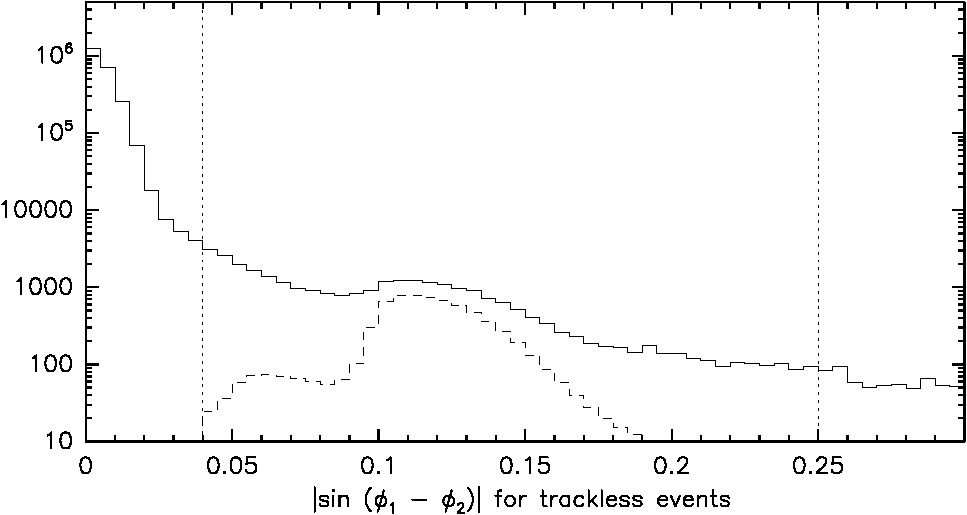
\includegraphics[width=\linewidth]{plots/runbyrun_trackless0}
  \caption{\label{runbyrun_trackless0} Back-to-backness in $\phi$ of
    two largest showers, in events with zero tracks.  The large peak at
    zero are gamgams and the little bump at 0.11 are trackless bhabhas.
    The dashed line shows two-track bhabhas for comparison, and the
    dotted lines are the cut boundaries for trackless bhabhas.}
\end{figure}

\begin{figure}[p]
  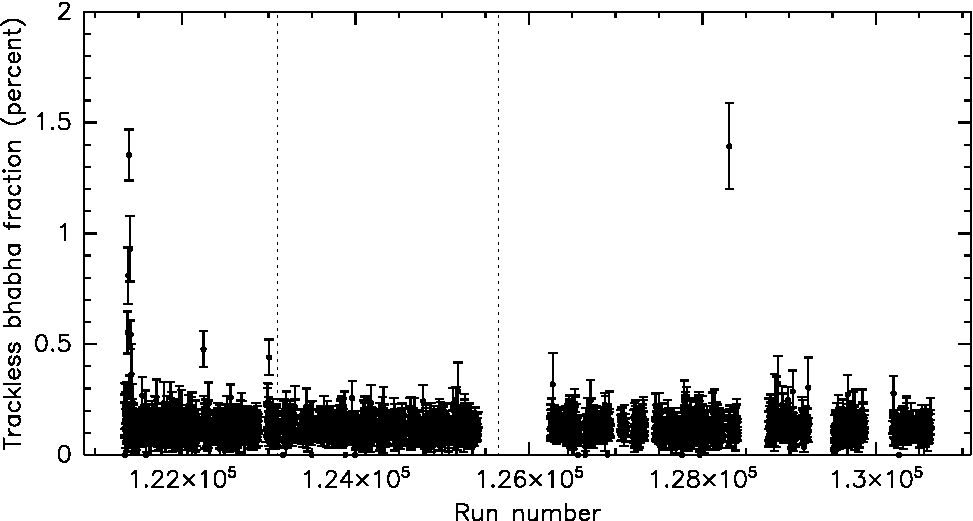
\includegraphics[width=\linewidth]{plots/runbyrun_trackless}
  \caption{\label{runbyrun_trackless} Trackless bhabha fraction (as a
  percent) for every run in the database dataset.  Dotted lines
  separate $\Upsilon(3S)$, $\Upsilon(1S)$, and $\Upsilon(2S)$ (left to
  right).}
\end{figure}

Of these twenty-five outliers, ten are scan runs, which are too
valuable to this analysis to lose.  Therefore, these ten runs were
retained and the other fifteen were rejected before plotting Figure
\ref{runbyrun_trackless}.  (The rejected runs are listed in Table
\ref{datasets:badruns}.)  All of the ten scan runs that had DR
problems had them in the last one-hundredth of the run, as seen in
Figure \ref{runbyrun_trackless2}.  When I count hadrons and gamgams
for these runs, I must count them in only the first 99\% of the run.

\begin{figure}[p]
  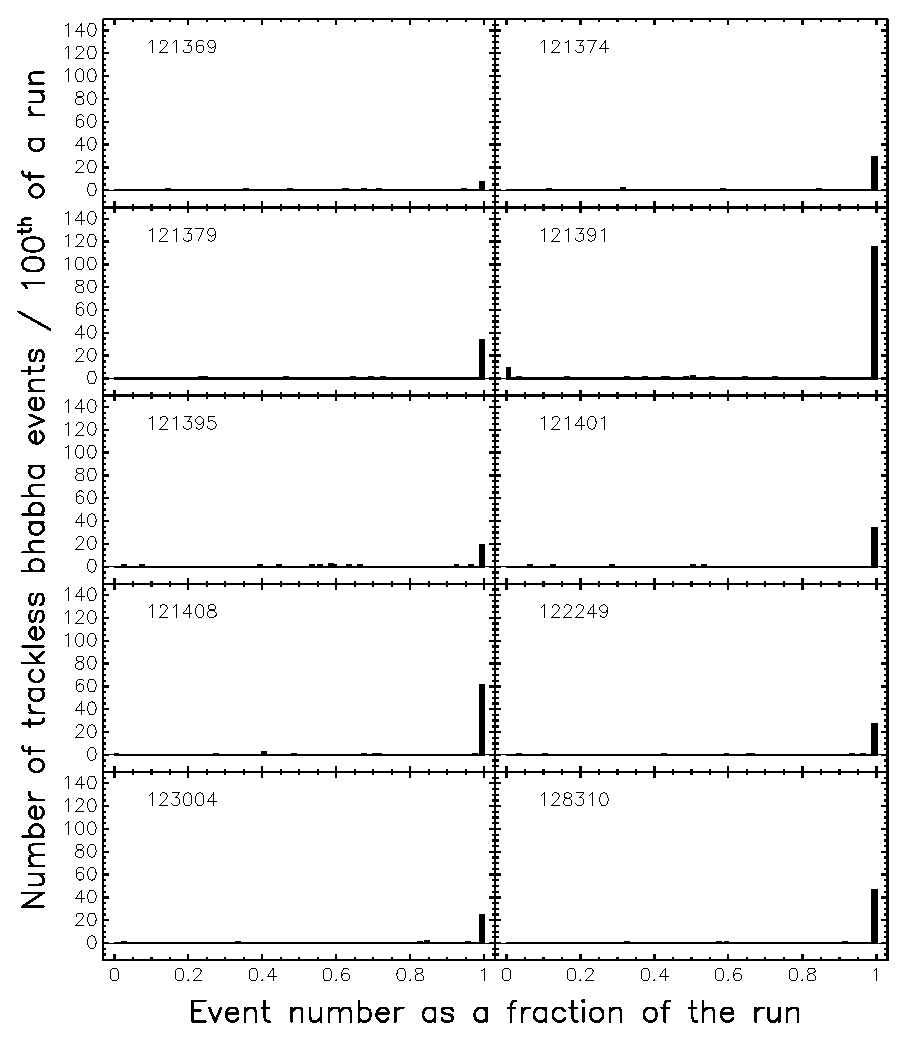
\includegraphics[width=\linewidth]{plots/runbyrun_trackless2}
  \caption{\label{runbyrun_trackless2} Number of trackless bhabhas
  throughout the run for the eight outliers in Figure
  \ref{runbyrun_trackless}.  Histograms are shaded black for
  visibility.}
\end{figure}

\section{Checking for CC Failures}

To check for CC failures, I created the event types DR-trigger bhabha
and DR-trigger mupair.  Both of these require the TwoTrack trigger
only, in order to be independent of the CC, and are built from the
same set of track requirements.  The only difference between these two
event types (and the only reference to a CC variable) is that the
DR-trigger bhabhas require \etwo\ $>$ 40\% \ebeam\ (which is loose)
and DR-trigger mupairs require \etwo\ $<$ 1 GeV.  (These are
non-overlapping criteria.)  This way, if the CC fails, bhabhas will be
identified as mupairs.

The $e^+e^-$ rate, given these cuts, is 13 to 19 times the
$\mu^+\mu^-$ rate, depending on whether the run is on the
$\Upsilon(1S)$ resonance (which contributes fractionally more to the
$\mu^+\mu^-$ rate than to the $e^+e^-$ rate) or in the continuum.
Therefore, a 13\% excess in the ratio
\begin{equation}
  \frac{\mbox{\#DR-trigger mupair}}{\mbox{\#DR-trigger bhabha +
  \#DR-trigger mupair}}
\end{equation}
is a 1\% limit on the fraction of time that the CC is insensitive.
This is because the denominator is independent of CC sensitivity and
CC failures add bhabhas to the mupair count.  I will call this ratio
the mupair fraction.

The mupair fraction is plotted for every run in the database dataset
in Figure \ref{runbyrun_bhamutt}.  No outliers are apparent, but the
statistical uncertainty is too large to place a tight and rigorous
limit on CC failures.  The excess ``mupairs'' in a given run is at
most about 50\%, which translates to a 4\% upper limit on the fraction
of time that the CC is insensitive in a given run.  This is comparable
with the statistical error in hadronic cross-section for a typical
run.

\begin{figure}[p]
  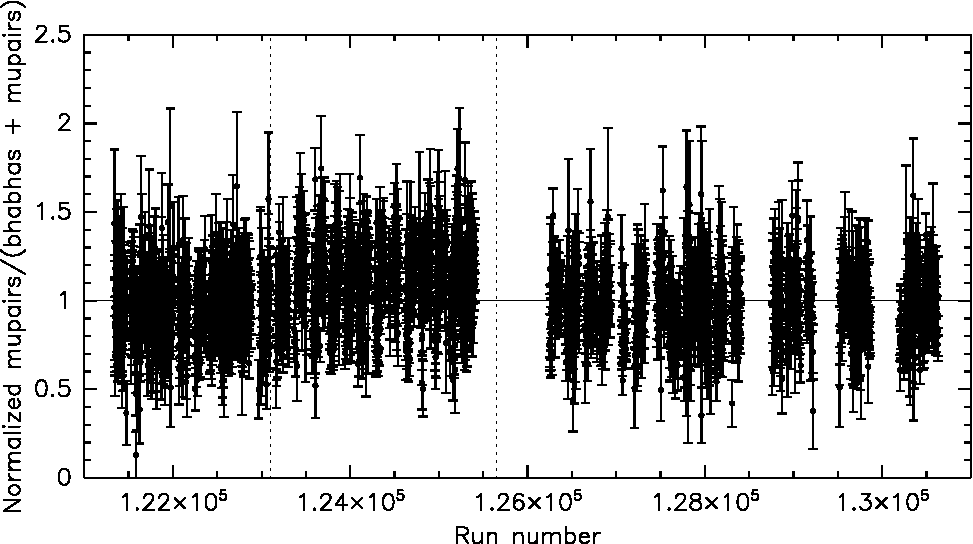
\includegraphics[width=\linewidth]{plots/runbyrun_bhamutt}
  \caption{\label{runbyrun_bhamutt} The mupair fraction, normalized to
  have a weighted mean of 1.0, plotted for every run in the database
  dataset.  Dotted lines separate $\Upsilon(3S)$, $\Upsilon(1S)$, and
  $\Upsilon(2S)$ (left to right).}
\end{figure}

\begin{figure}[p]
  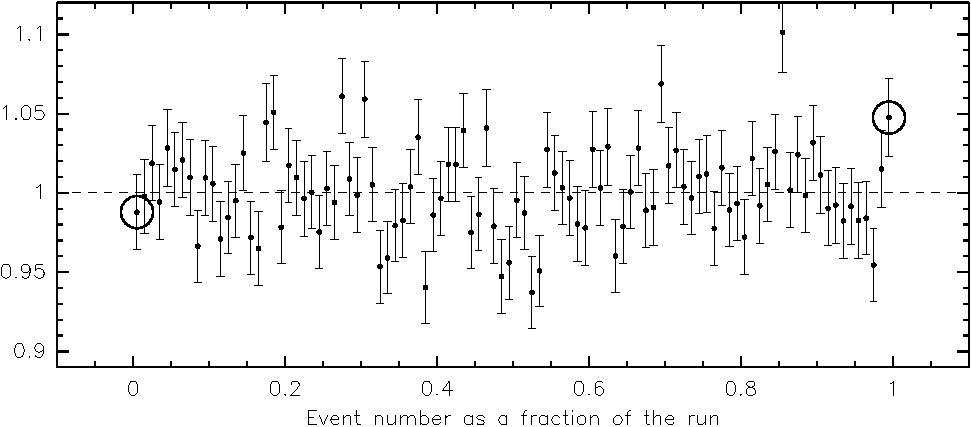
\includegraphics[width=\linewidth]{plots/runbyrun_bhamutt2}
  \caption{\label{runbyrun_bhamutt2} Mupair fraction throughout the
    run, where all runs have been combined.  The first and last bins
    (circled) do not deviate significantly from the average.}
\end{figure}

Assuming, as was the case for DR failures, that detector failure
either happens at the very beginning or the very end of a run, I
plotted the mupair fraction as a function of the run, and combined all
runs together.  In the resulting histogram, the first bin represents
the first hundredth of every run, and the last bin represents the last
hundredth of every run.  If there are CC failures that always happen
at the beginning or the end of the run, they will pile up in these two
bins and I will see a deviation.  The biggest detectable deviations
are 2.7\% for the first hundredth and 5.4\% for the last hundredth
(deviation and uncertainty added in quadrature).  These translate to
0.2\% and 0.4\% limits on the total CC failure rate (good runs
included).  This histogram is plotted in Figure
\ref{runbyrun_bhamutt2}.

Scanning through many of these histograms for individual runs, I did
not see anything peculiar.  I will assume that while the DR can lose
high voltage with the CC still taking data, the CC cannot lose
sensitivity while the DR is still taking data.

\section{Relative Hadronic Cross-section}

Now I am ready to calculate the relative hadronic cross-section.  By
``relative,'' I mean that I will not apply the hadronic efficiency
correction or translate the number of gamgams into an integrated
luminosity in inverse nanobarns: I will just divide the hadron count
by the gamgam count.  I do, however, make corrections that depend on
run number.  The gamgam count has been corrected for BarrelBhabha
trigger efficiency, and the hadron count has been beam-gas-subtracted
(50\% correction with 50\% uncertainty) and cosmic ray-subtracted
(only statistical errors).  In Subsection \ref{runbyrun_ssecvsenergy},
I will also divide by $s$ = \ebeam$^2$ so that hadronic cross-sections
at different energies may be compared.

\subsection{Throughout Each Run}

In presenting relative hadronic cross-sections, I will start at the
most instrumental level and work up to fundamental physics.  First I
plot hadronic cross-section within each run.  Every run was taken at
exactly one beam energy, so this should be constant.  As I did in the
DR and CC tests, I can calculate the hadronic cross-section for each
hundredth of a run, and then perform linear fits to hadronic
cross-section versus time.  The slope of each fit is divided by its
uncertainty and these ``pulls'' are histogrammed in Figure
\ref{runbyrun_hadxs1}-a.  The average slope is zero with only
statistical deviations.  The $\chi^2$ of the linear fits is another
way to spot misshapen distributions: the reduced $\chi^2$ for all the
fits is histogrammed in Figure
\ref{runbyrun_hadxs1}-b.  The average reduced $\chi^2$ is low, but
this may be an effect propagated from low-statistics bins in the
gamgam versus time histograms.

Before drawing these histograms, two outlying runs were identified:
their hadronic cross-section versus time plots are shown in Figure
\ref{runbyrun_hadxs2}.  They have been removed from the dataset.

\begin{figure}[p]
  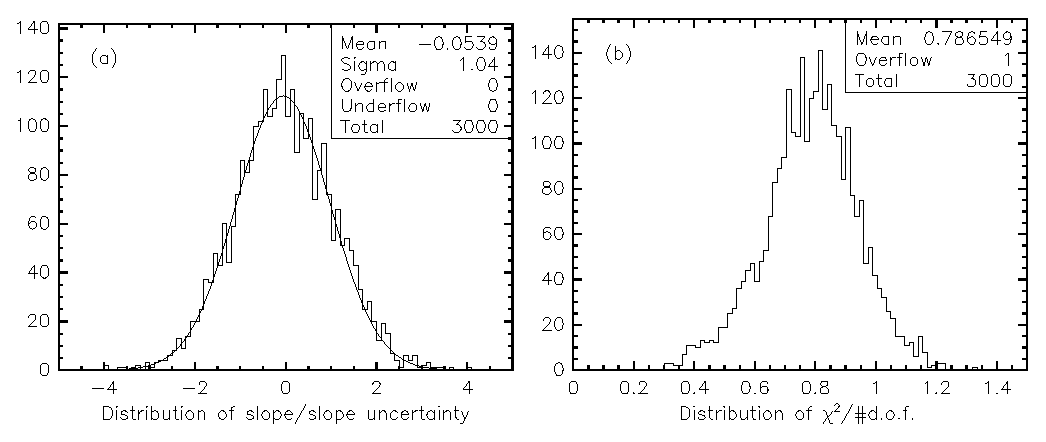
\includegraphics[width=\linewidth]{plots/runbyrun_hadxs1}
  \caption{\label{runbyrun_hadxs1} From left to right: (a) pull
  distribution of slopes in the hadronic cross-section versus time
  fits, as a number of sigmas from zero, and (b) distribution of
  reduced $\chi^2$ for the same fits.  (The outlier is a statistical
  variant.)}
\end{figure}

\begin{figure}[p]
  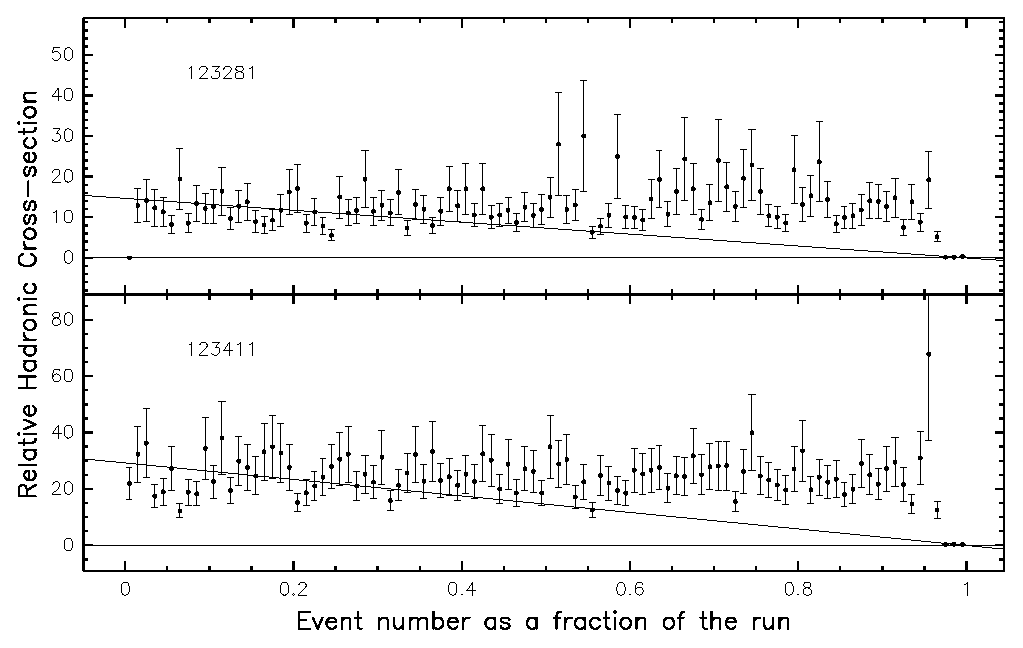
\includegraphics[width=\linewidth]{plots/runbyrun_hadxs2}
  \caption{\label{runbyrun_hadxs2} Two runs that failed to have a
  satisfactory slope (not included in the histograms in Figure
  \ref{runbyrun_hadxs1})}
\end{figure}

\subsection{Run by Run}

Next I will plot the hadronic cross section for each on- and
off-resonance run in the database dataset.  Each of these six samples
(three resonances times on- versus off-resonance) was taken at a
constant beam energy, so the hadronic cross-section should be
constant.  The definition of ``on-resonance'' is a range of energies
only 1.6 MeV wide for each resonance, so this, too, should be
constant.  No $1/s$ correction has been applied in this Subsection, so
continua at the $\Upsilon(1S)$, $\Upsilon(2S)$, and $\Upsilon(3S)$
should all have equal values.  The plots are shown in Figure
\ref{runbyrun_peaksconts}.

\begin{figure}[p]
  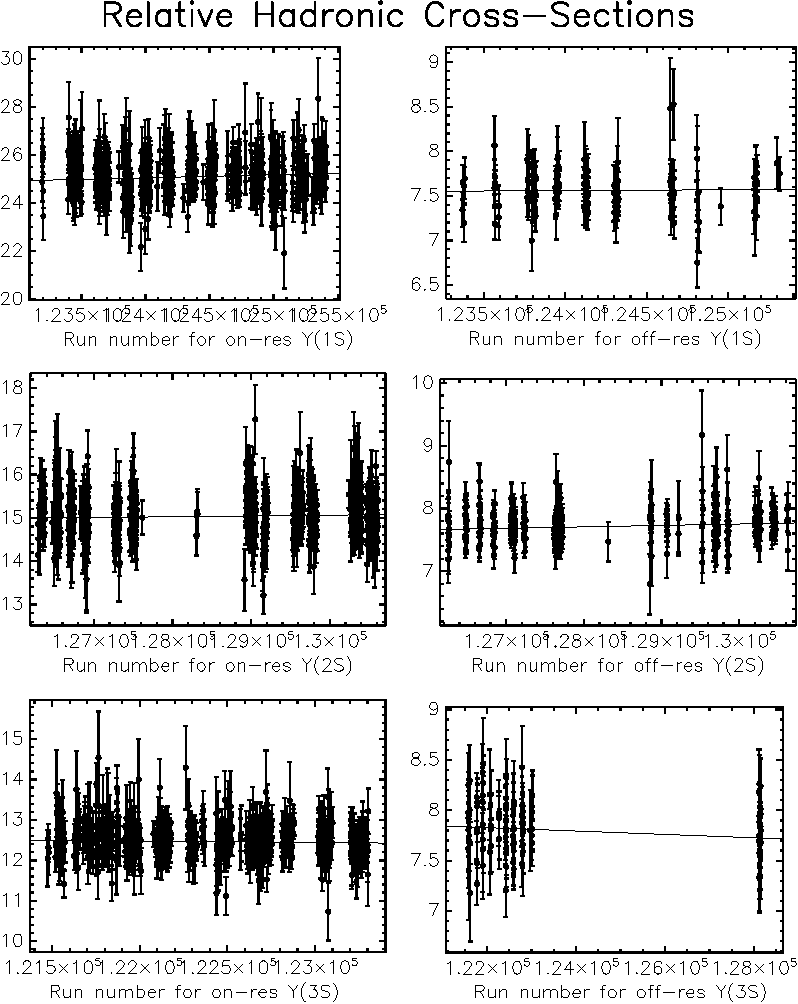
\includegraphics[width=\linewidth]{plots/runbyrun_peaksconts}
  \caption{\label{runbyrun_peaksconts} Relative hadronic cross-section
    versus run number for each of the six constant energies.  A
    straight line has been fitted to each.}
\end{figure}

\begin{figure}[p]
  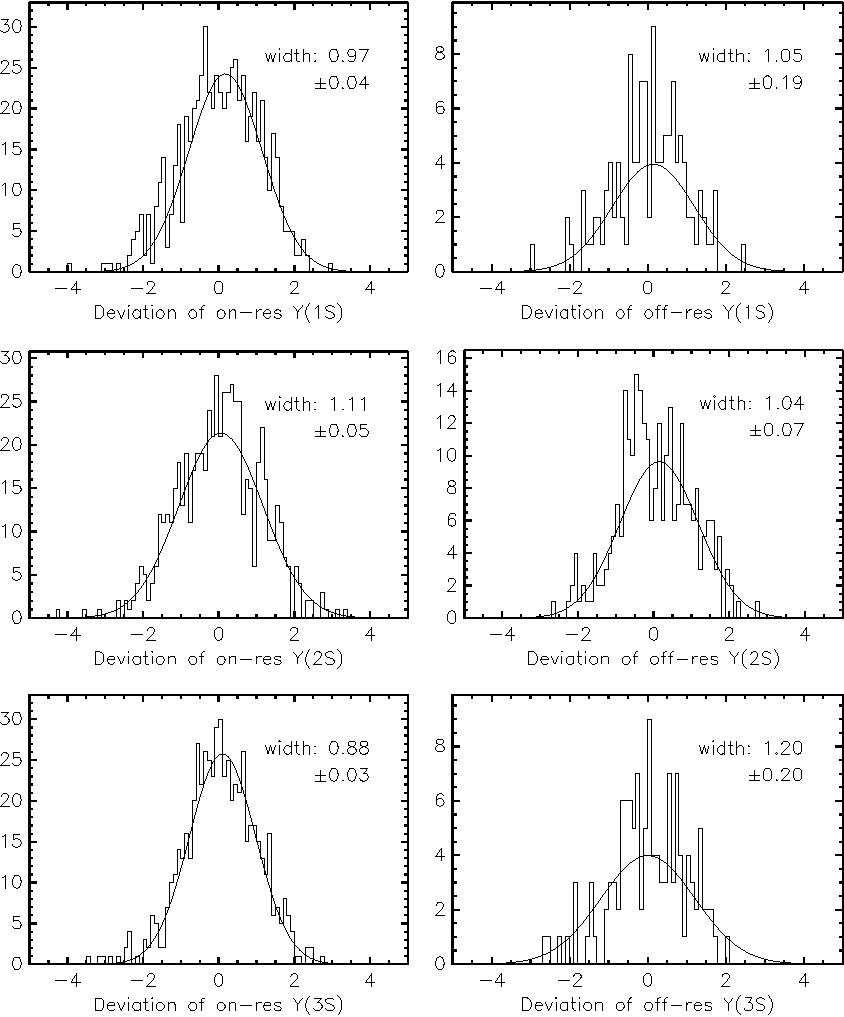
\includegraphics[width=\linewidth]{plots/runbyrun_peaksconts2}
  \caption{\label{runbyrun_peaksconts2} Pull distributions of hadronic
  cross-section in each constant-energy sample.  The widths of fitted
  Gaussians are also displayed.}
\end{figure}

I fitted each constant hadronic cross-section with a straight line.
The significance (value divided by error) of each slope is:
\begin{center}
  \begin{tabular}{c c c c}
    & on-resonance & off-resonance \\
    $\Upsilon(1S)$ & 3.13 & 0.25 \\
    $\Upsilon(2S)$ & 1.76 & 2.45 \\
    $\Upsilon(3S)$ & -1.32 & -1.77. \\
  \end{tabular}
\end{center}
Some of these are marginally significant, so I should try to match
peak and scan data with nearby continuum as much as possible, such
that varying continuum levels are subtracted in a way that cancels the
drift.

Scan and continuum runs aren't always consecutive in the
$\Upsilon(2S)$ dataset, so I will be forced to use continuum from
different eras for a continuum subtraction.  However, at run 127642,
the CC begins to intermittently read out some showers (along the tile
boundaries in the barrel) with higher energies than it should.  This
could raise the hadron count because two-photon events, which are
normally cut out for having too little \visen, may be artificially
raised above the cut threshold.  In fact, combining all $\Upsilon(2S)$
peak and continuum, before and after 127642, I see the peak data raise
2.49 standard deviations (0.078 $\pm$ 0.031 in \#hadrons/\#gamgams
units) and the continuum raise 1.56 standard deviations (0.042 $\pm$
0.027 in the same units).  I will avoid crossing this boundary for
continuum-subtractions.

%% peak
%% (14.991370234331351, 0.024844739090064256)
%% (15.069660152908128, 0.019256898584188539)
%% 0.078 +- 0.031  is 2.49 sigmas

%% cont
%% (7.6884592194542147, 0.020992094512067197)
%% (7.7303710804873385, 0.016947379302405009)
%% 0.042 +- 0.027  is 1.56 sigmas

%% peak bhabha
%% (1.1453608108322908, 0.00069472852035430026)
%% (1.1514073256621737, 0.00053750979311212863)

%% cont bhabha
%% (59.556019903921154, 0.069744336836371058)
%% (59.524565678673258, 0.055778459450481861)
%% 0.031 +- 0.089  is 0.35 sigmas

The $\Upsilon(3S)$ off-resonance dataset has a very large gap before
its last group of runs: extra $\Upsilon(3S)$ was acquired during
$\Upsilon(2S)$ running.  The late $\Upsilon(3S)$ sample includes runs
that are near the peak, but not close enough for my classification.
They have been labeled ``scan'' runs.  I won't mix late $\Upsilon(3S)$
with early $\Upsilon(3S)$.

As a last consistency check, I calculate how far each run is from the
weighted mean of its class as a number of standard deviations.  The
resulting six pull distributions should each be unit Gaussians, and
most of them are, as can be seen in Figure \ref{runbyrun_peaksconts2}.
I cannot explain the narrow width of the $\Upsilon(3S)$.

\subsection{Versus Energy} \label{runbyrun_ssecvsenergy}

Finally, the physics: I will now plot hadronic cross-section as a
function of center-of-mass energy.  To do this properly, I will need
to multiply $\mbox{\#hadrons}/\mbox{\#gamgams}$ by a factor of $1/s$.
The plot of all hadronic cross-sections versus energy is in Figure
\ref{runbyrun_thescans}.  The (nearly) horizontal line on all three
plots is a $1/s$ fit to all continuum data simultaneously; the
$\chi^2/$\#d.o.f. of that fit is 554/525 = 1.06 (an 80\% confidence
level).

There appears to be a distortion in the $\Upsilon(3S)$ lineshape: the
runs responsible for this distortion are all from an era before the
first (intentional) $\Upsilon(3S)$ scan.  In the following Chapter, I
will determine the dates when alterations to the beam energy
calibration are likely to have taken place: the runs responsible for
this distortion may be before the first such calibration, and their
energies therefore can't be determined.  Data like these will not be a
part of any lineshape fit.

\begin{figure}[p]
  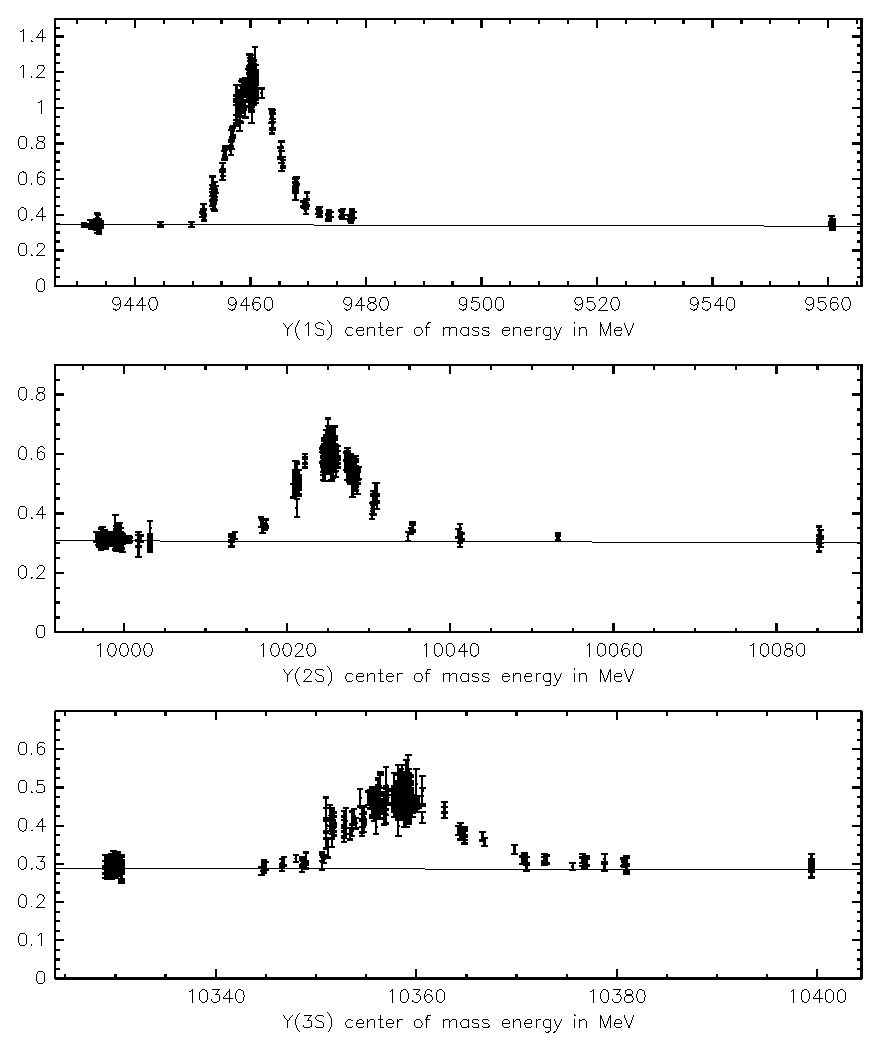
\includegraphics[width=\linewidth]{plots/runbyrun_thescans}
  \caption{\label{runbyrun_thescans} Relative hadronic cross-section
  versus energy reveals the $\Upsilon$ resonance peaks.  The (nearly)
  horizontal line is a $1/s$ fit to all continuum data.}
\end{figure}
